%==============================================================================
% Figure: Fractal Hausdorff Dimension (Koch Snowflake)
% Source: Ch05 (Fractal Calculus)
% Framework: M (Mathematical) | Type: Iterative construction diagram
% Date: 2025-10-21
%==============================================================================

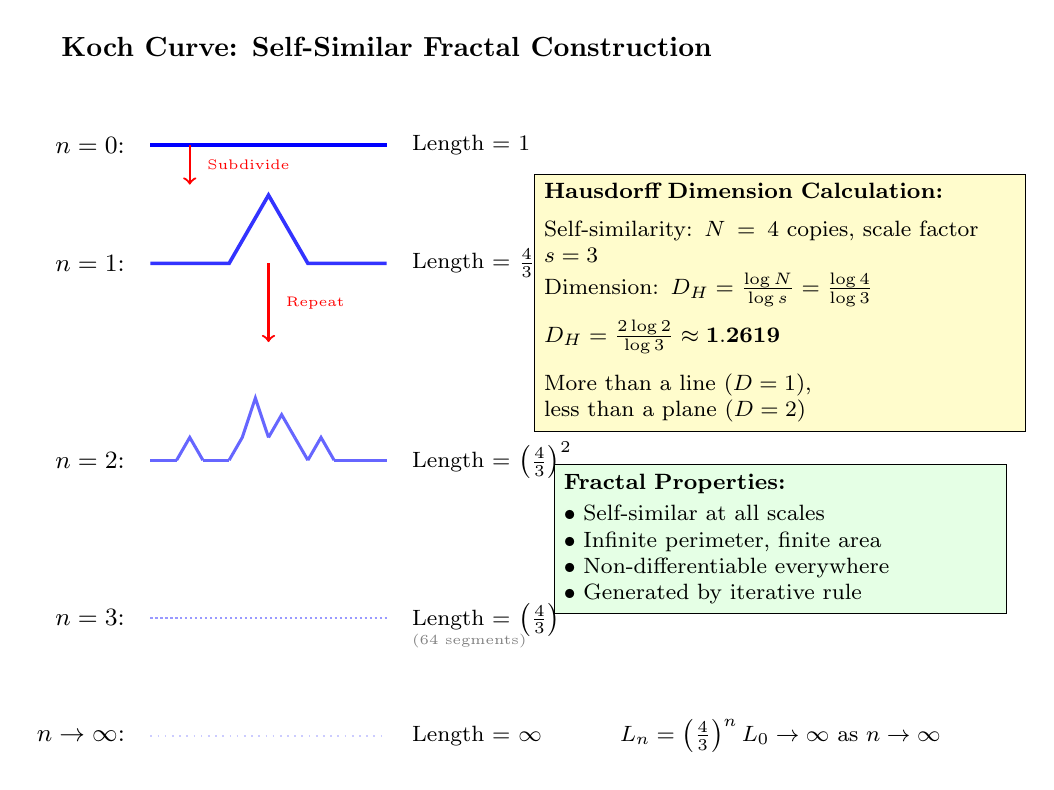
\begin{tikzpicture}[scale=1.0]
  % Title
  \node[anchor=north] at (3,8.5) {\textbf{Koch Curve: Self-Similar Fractal Construction}};

  % Iteration 0 (base line)
  \draw[line width=1.5pt, blue] (0,7) -- (3,7);
  \node[anchor=east, font=\small] at (-0.2,7) {$n=0$:};
  \node[anchor=west, font=\footnotesize] at (3.2,7) {Length = 1};

  % Iteration 1
  \draw[line width=1.3pt, blue!80] (0,5.5) -- (1,5.5) -- (1.5,6.366) -- (2,5.5) -- (3,5.5);
  \node[anchor=east, font=\small] at (-0.2,5.5) {$n=1$:};
  \node[anchor=west, font=\footnotesize] at (3.2,5.5) {Length = $\frac{4}{3}$};

  % Iteration 2 (simplified representation)
  \begin{scope}[yshift=-2.5cm]
    \draw[line width=1.1pt, blue!60] (0,5.5) -- (0.333,5.5);
    \draw[line width=1.1pt, blue!60] (0.333,5.5) -- (0.5,5.789) -- (0.667,5.5);
    \draw[line width=1.1pt, blue!60] (0.667,5.5) -- (1,5.5);
    \draw[line width=1.1pt, blue!60] (1,5.5) -- (1.167,5.789) -- (1.333,6.289) -- (1.5,5.789);
    \draw[line width=1.1pt, blue!60] (1.5,5.789) -- (1.667,6.078) -- (1.833,5.789);
    \draw[line width=1.1pt, blue!60] (1.833,5.789) -- (2,5.5);
    \draw[line width=1.1pt, blue!60] (2,5.5) -- (2.167,5.789) -- (2.333,5.5);
    \draw[line width=1.1pt, blue!60] (2.333,5.5) -- (3,5.5);
    \node[anchor=east, font=\small] at (-0.2,5.5) {$n=2$:};
    \node[anchor=west, font=\footnotesize] at (3.2,5.5) {Length = $\left(\frac{4}{3}\right)^2$};
  \end{scope}

  % Iteration 3 (highly detailed, stylized)
  \node[anchor=east, font=\small] at (-0.2,1) {$n=3$:};
  \draw[line width=0.8pt, blue!40, densely dotted] (0,1) -- (3,1);
  \node[anchor=west, font=\footnotesize] at (3.2,1) {Length = $\left(\frac{4}{3}\right)^3$};
  \node[anchor=west, font=\tiny, text=gray] at (3.2,0.7) {(64 segments)};

  % Iteration infinity
  \node[anchor=east, font=\small] at (-0.2,-0.5) {$n\to\infty$:};
  \draw[line width=0.6pt, blue!20, dotted] (0,-0.5) -- (3,-0.5);
  \node[anchor=west, font=\footnotesize] at (3.2,-0.5) {Length = $\infty$};

  % Hausdorff dimension calculation box
  \node[draw, rectangle, fill=yellow!20, font=\footnotesize, align=left, text width=6cm] at (8,5) {
    \textbf{Hausdorff Dimension Calculation:} \\[4pt]
    Self-similarity: $N = 4$ copies, scale factor $s = 3$ \\[2pt]
    Dimension: $D_H = \frac{\log N}{\log s} = \frac{\log 4}{\log 3}$ \\[4pt]
    $D_H = \frac{2\log 2}{\log 3} \approx \mathbf{1.2619}$ \\[6pt]
    More than a line ($D=1$), \\
    less than a plane ($D=2$)
  };

  % Visual proof of self-similarity
  \draw[thick, red, ->] (0.5,7) -- (0.5,6.5);
  \node[anchor=west, font=\tiny, text=red] at (0.6,6.75) {Subdivide};

  \draw[thick, red, ->] (1.5,5.5) -- (1.5,4.5);
  \node[anchor=west, font=\tiny, text=red] at (1.6,5) {Repeat};

  % Property box
  \node[draw, rectangle, fill=green!10, font=\footnotesize, align=left, text width=5.5cm] at (8,2) {
    \textbf{Fractal Properties:} \\[2pt]
    $\bullet$ Self-similar at all scales \\
    $\bullet$ Infinite perimeter, finite area \\
    $\bullet$ Non-differentiable everywhere \\
    $\bullet$ Generated by iterative rule
  };

  % Length scaling formula
  \node[font=\footnotesize] at (8,-0.5) {
    $L_n = \left(\frac{4}{3}\right)^n L_0 \to \infty$ as $n \to \infty$
  };

\end{tikzpicture}

% Usage: %==============================================================================
% Figure: Fractal Hausdorff Dimension (Koch Snowflake)
% Source: Ch05 (Fractal Calculus)
% Framework: M (Mathematical) | Type: Iterative construction diagram
% Date: 2025-10-21
%==============================================================================

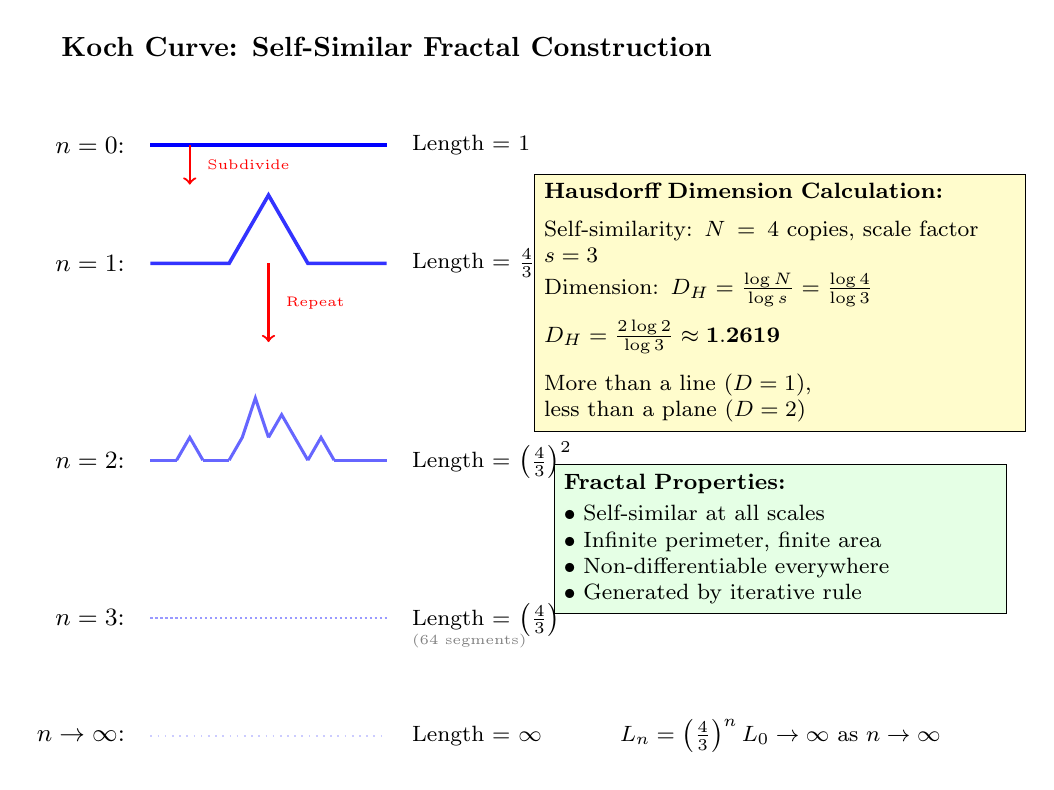
\begin{tikzpicture}[scale=1.0]
  % Title
  \node[anchor=north] at (3,8.5) {\textbf{Koch Curve: Self-Similar Fractal Construction}};

  % Iteration 0 (base line)
  \draw[line width=1.5pt, blue] (0,7) -- (3,7);
  \node[anchor=east, font=\small] at (-0.2,7) {$n=0$:};
  \node[anchor=west, font=\footnotesize] at (3.2,7) {Length = 1};

  % Iteration 1
  \draw[line width=1.3pt, blue!80] (0,5.5) -- (1,5.5) -- (1.5,6.366) -- (2,5.5) -- (3,5.5);
  \node[anchor=east, font=\small] at (-0.2,5.5) {$n=1$:};
  \node[anchor=west, font=\footnotesize] at (3.2,5.5) {Length = $\frac{4}{3}$};

  % Iteration 2 (simplified representation)
  \begin{scope}[yshift=-2.5cm]
    \draw[line width=1.1pt, blue!60] (0,5.5) -- (0.333,5.5);
    \draw[line width=1.1pt, blue!60] (0.333,5.5) -- (0.5,5.789) -- (0.667,5.5);
    \draw[line width=1.1pt, blue!60] (0.667,5.5) -- (1,5.5);
    \draw[line width=1.1pt, blue!60] (1,5.5) -- (1.167,5.789) -- (1.333,6.289) -- (1.5,5.789);
    \draw[line width=1.1pt, blue!60] (1.5,5.789) -- (1.667,6.078) -- (1.833,5.789);
    \draw[line width=1.1pt, blue!60] (1.833,5.789) -- (2,5.5);
    \draw[line width=1.1pt, blue!60] (2,5.5) -- (2.167,5.789) -- (2.333,5.5);
    \draw[line width=1.1pt, blue!60] (2.333,5.5) -- (3,5.5);
    \node[anchor=east, font=\small] at (-0.2,5.5) {$n=2$:};
    \node[anchor=west, font=\footnotesize] at (3.2,5.5) {Length = $\left(\frac{4}{3}\right)^2$};
  \end{scope}

  % Iteration 3 (highly detailed, stylized)
  \node[anchor=east, font=\small] at (-0.2,1) {$n=3$:};
  \draw[line width=0.8pt, blue!40, densely dotted] (0,1) -- (3,1);
  \node[anchor=west, font=\footnotesize] at (3.2,1) {Length = $\left(\frac{4}{3}\right)^3$};
  \node[anchor=west, font=\tiny, text=gray] at (3.2,0.7) {(64 segments)};

  % Iteration infinity
  \node[anchor=east, font=\small] at (-0.2,-0.5) {$n\to\infty$:};
  \draw[line width=0.6pt, blue!20, dotted] (0,-0.5) -- (3,-0.5);
  \node[anchor=west, font=\footnotesize] at (3.2,-0.5) {Length = $\infty$};

  % Hausdorff dimension calculation box
  \node[draw, rectangle, fill=yellow!20, font=\footnotesize, align=left, text width=6cm] at (8,5) {
    \textbf{Hausdorff Dimension Calculation:} \\[4pt]
    Self-similarity: $N = 4$ copies, scale factor $s = 3$ \\[2pt]
    Dimension: $D_H = \frac{\log N}{\log s} = \frac{\log 4}{\log 3}$ \\[4pt]
    $D_H = \frac{2\log 2}{\log 3} \approx \mathbf{1.2619}$ \\[6pt]
    More than a line ($D=1$), \\
    less than a plane ($D=2$)
  };

  % Visual proof of self-similarity
  \draw[thick, red, ->] (0.5,7) -- (0.5,6.5);
  \node[anchor=west, font=\tiny, text=red] at (0.6,6.75) {Subdivide};

  \draw[thick, red, ->] (1.5,5.5) -- (1.5,4.5);
  \node[anchor=west, font=\tiny, text=red] at (1.6,5) {Repeat};

  % Property box
  \node[draw, rectangle, fill=green!10, font=\footnotesize, align=left, text width=5.5cm] at (8,2) {
    \textbf{Fractal Properties:} \\[2pt]
    $\bullet$ Self-similar at all scales \\
    $\bullet$ Infinite perimeter, finite area \\
    $\bullet$ Non-differentiable everywhere \\
    $\bullet$ Generated by iterative rule
  };

  % Length scaling formula
  \node[font=\footnotesize] at (8,-0.5) {
    $L_n = \left(\frac{4}{3}\right)^n L_0 \to \infty$ as $n \to \infty$
  };

\end{tikzpicture}

% Usage: %==============================================================================
% Figure: Fractal Hausdorff Dimension (Koch Snowflake)
% Source: Ch05 (Fractal Calculus)
% Framework: M (Mathematical) | Type: Iterative construction diagram
% Date: 2025-10-21
%==============================================================================

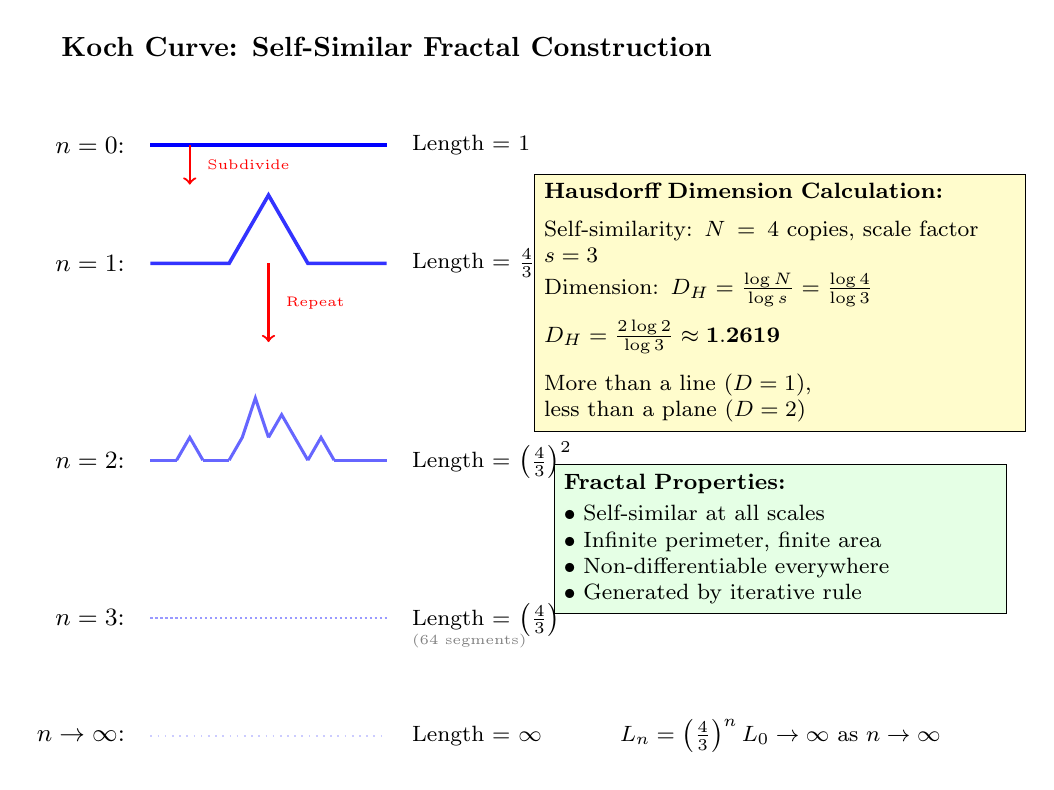
\begin{tikzpicture}[scale=1.0]
  % Title
  \node[anchor=north] at (3,8.5) {\textbf{Koch Curve: Self-Similar Fractal Construction}};

  % Iteration 0 (base line)
  \draw[line width=1.5pt, blue] (0,7) -- (3,7);
  \node[anchor=east, font=\small] at (-0.2,7) {$n=0$:};
  \node[anchor=west, font=\footnotesize] at (3.2,7) {Length = 1};

  % Iteration 1
  \draw[line width=1.3pt, blue!80] (0,5.5) -- (1,5.5) -- (1.5,6.366) -- (2,5.5) -- (3,5.5);
  \node[anchor=east, font=\small] at (-0.2,5.5) {$n=1$:};
  \node[anchor=west, font=\footnotesize] at (3.2,5.5) {Length = $\frac{4}{3}$};

  % Iteration 2 (simplified representation)
  \begin{scope}[yshift=-2.5cm]
    \draw[line width=1.1pt, blue!60] (0,5.5) -- (0.333,5.5);
    \draw[line width=1.1pt, blue!60] (0.333,5.5) -- (0.5,5.789) -- (0.667,5.5);
    \draw[line width=1.1pt, blue!60] (0.667,5.5) -- (1,5.5);
    \draw[line width=1.1pt, blue!60] (1,5.5) -- (1.167,5.789) -- (1.333,6.289) -- (1.5,5.789);
    \draw[line width=1.1pt, blue!60] (1.5,5.789) -- (1.667,6.078) -- (1.833,5.789);
    \draw[line width=1.1pt, blue!60] (1.833,5.789) -- (2,5.5);
    \draw[line width=1.1pt, blue!60] (2,5.5) -- (2.167,5.789) -- (2.333,5.5);
    \draw[line width=1.1pt, blue!60] (2.333,5.5) -- (3,5.5);
    \node[anchor=east, font=\small] at (-0.2,5.5) {$n=2$:};
    \node[anchor=west, font=\footnotesize] at (3.2,5.5) {Length = $\left(\frac{4}{3}\right)^2$};
  \end{scope}

  % Iteration 3 (highly detailed, stylized)
  \node[anchor=east, font=\small] at (-0.2,1) {$n=3$:};
  \draw[line width=0.8pt, blue!40, densely dotted] (0,1) -- (3,1);
  \node[anchor=west, font=\footnotesize] at (3.2,1) {Length = $\left(\frac{4}{3}\right)^3$};
  \node[anchor=west, font=\tiny, text=gray] at (3.2,0.7) {(64 segments)};

  % Iteration infinity
  \node[anchor=east, font=\small] at (-0.2,-0.5) {$n\to\infty$:};
  \draw[line width=0.6pt, blue!20, dotted] (0,-0.5) -- (3,-0.5);
  \node[anchor=west, font=\footnotesize] at (3.2,-0.5) {Length = $\infty$};

  % Hausdorff dimension calculation box
  \node[draw, rectangle, fill=yellow!20, font=\footnotesize, align=left, text width=6cm] at (8,5) {
    \textbf{Hausdorff Dimension Calculation:} \\[4pt]
    Self-similarity: $N = 4$ copies, scale factor $s = 3$ \\[2pt]
    Dimension: $D_H = \frac{\log N}{\log s} = \frac{\log 4}{\log 3}$ \\[4pt]
    $D_H = \frac{2\log 2}{\log 3} \approx \mathbf{1.2619}$ \\[6pt]
    More than a line ($D=1$), \\
    less than a plane ($D=2$)
  };

  % Visual proof of self-similarity
  \draw[thick, red, ->] (0.5,7) -- (0.5,6.5);
  \node[anchor=west, font=\tiny, text=red] at (0.6,6.75) {Subdivide};

  \draw[thick, red, ->] (1.5,5.5) -- (1.5,4.5);
  \node[anchor=west, font=\tiny, text=red] at (1.6,5) {Repeat};

  % Property box
  \node[draw, rectangle, fill=green!10, font=\footnotesize, align=left, text width=5.5cm] at (8,2) {
    \textbf{Fractal Properties:} \\[2pt]
    $\bullet$ Self-similar at all scales \\
    $\bullet$ Infinite perimeter, finite area \\
    $\bullet$ Non-differentiable everywhere \\
    $\bullet$ Generated by iterative rule
  };

  % Length scaling formula
  \node[font=\footnotesize] at (8,-0.5) {
    $L_n = \left(\frac{4}{3}\right)^n L_0 \to \infty$ as $n \to \infty$
  };

\end{tikzpicture}

% Usage: %==============================================================================
% Figure: Fractal Hausdorff Dimension (Koch Snowflake)
% Source: Ch05 (Fractal Calculus)
% Framework: M (Mathematical) | Type: Iterative construction diagram
% Date: 2025-10-21
%==============================================================================

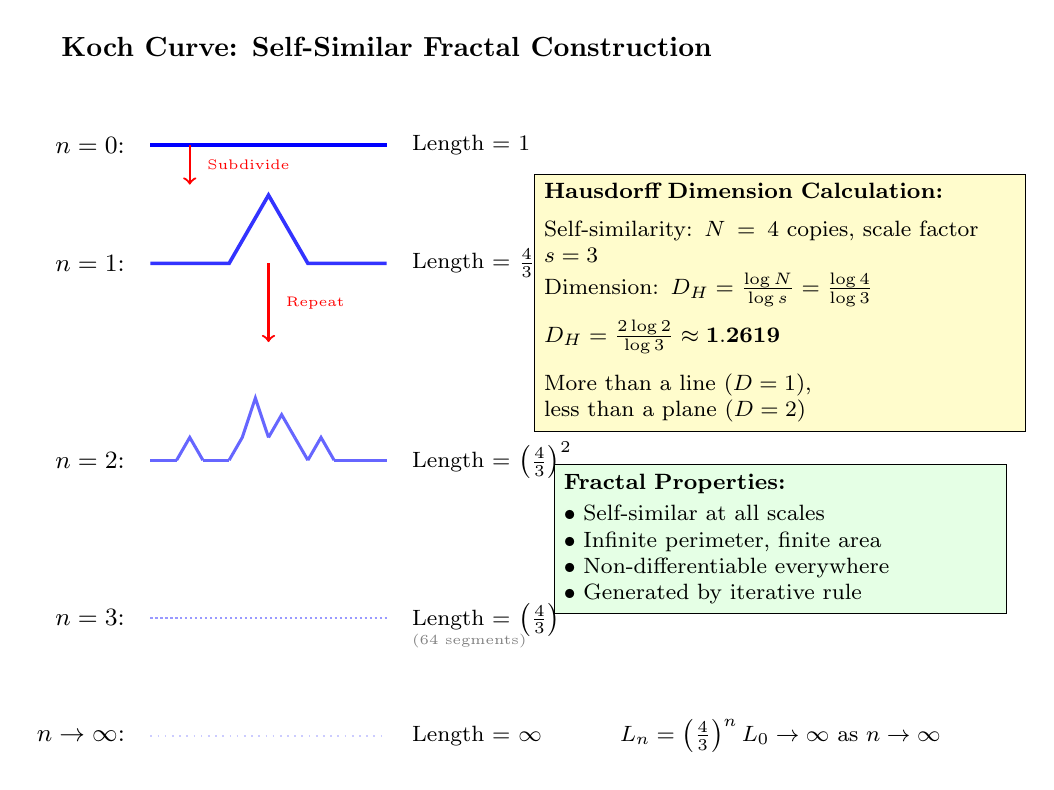
\begin{tikzpicture}[scale=1.0]
  % Title
  \node[anchor=north] at (3,8.5) {\textbf{Koch Curve: Self-Similar Fractal Construction}};

  % Iteration 0 (base line)
  \draw[line width=1.5pt, blue] (0,7) -- (3,7);
  \node[anchor=east, font=\small] at (-0.2,7) {$n=0$:};
  \node[anchor=west, font=\footnotesize] at (3.2,7) {Length = 1};

  % Iteration 1
  \draw[line width=1.3pt, blue!80] (0,5.5) -- (1,5.5) -- (1.5,6.366) -- (2,5.5) -- (3,5.5);
  \node[anchor=east, font=\small] at (-0.2,5.5) {$n=1$:};
  \node[anchor=west, font=\footnotesize] at (3.2,5.5) {Length = $\frac{4}{3}$};

  % Iteration 2 (simplified representation)
  \begin{scope}[yshift=-2.5cm]
    \draw[line width=1.1pt, blue!60] (0,5.5) -- (0.333,5.5);
    \draw[line width=1.1pt, blue!60] (0.333,5.5) -- (0.5,5.789) -- (0.667,5.5);
    \draw[line width=1.1pt, blue!60] (0.667,5.5) -- (1,5.5);
    \draw[line width=1.1pt, blue!60] (1,5.5) -- (1.167,5.789) -- (1.333,6.289) -- (1.5,5.789);
    \draw[line width=1.1pt, blue!60] (1.5,5.789) -- (1.667,6.078) -- (1.833,5.789);
    \draw[line width=1.1pt, blue!60] (1.833,5.789) -- (2,5.5);
    \draw[line width=1.1pt, blue!60] (2,5.5) -- (2.167,5.789) -- (2.333,5.5);
    \draw[line width=1.1pt, blue!60] (2.333,5.5) -- (3,5.5);
    \node[anchor=east, font=\small] at (-0.2,5.5) {$n=2$:};
    \node[anchor=west, font=\footnotesize] at (3.2,5.5) {Length = $\left(\frac{4}{3}\right)^2$};
  \end{scope}

  % Iteration 3 (highly detailed, stylized)
  \node[anchor=east, font=\small] at (-0.2,1) {$n=3$:};
  \draw[line width=0.8pt, blue!40, densely dotted] (0,1) -- (3,1);
  \node[anchor=west, font=\footnotesize] at (3.2,1) {Length = $\left(\frac{4}{3}\right)^3$};
  \node[anchor=west, font=\tiny, text=gray] at (3.2,0.7) {(64 segments)};

  % Iteration infinity
  \node[anchor=east, font=\small] at (-0.2,-0.5) {$n\to\infty$:};
  \draw[line width=0.6pt, blue!20, dotted] (0,-0.5) -- (3,-0.5);
  \node[anchor=west, font=\footnotesize] at (3.2,-0.5) {Length = $\infty$};

  % Hausdorff dimension calculation box
  \node[draw, rectangle, fill=yellow!20, font=\footnotesize, align=left, text width=6cm] at (8,5) {
    \textbf{Hausdorff Dimension Calculation:} \\[4pt]
    Self-similarity: $N = 4$ copies, scale factor $s = 3$ \\[2pt]
    Dimension: $D_H = \frac{\log N}{\log s} = \frac{\log 4}{\log 3}$ \\[4pt]
    $D_H = \frac{2\log 2}{\log 3} \approx \mathbf{1.2619}$ \\[6pt]
    More than a line ($D=1$), \\
    less than a plane ($D=2$)
  };

  % Visual proof of self-similarity
  \draw[thick, red, ->] (0.5,7) -- (0.5,6.5);
  \node[anchor=west, font=\tiny, text=red] at (0.6,6.75) {Subdivide};

  \draw[thick, red, ->] (1.5,5.5) -- (1.5,4.5);
  \node[anchor=west, font=\tiny, text=red] at (1.6,5) {Repeat};

  % Property box
  \node[draw, rectangle, fill=green!10, font=\footnotesize, align=left, text width=5.5cm] at (8,2) {
    \textbf{Fractal Properties:} \\[2pt]
    $\bullet$ Self-similar at all scales \\
    $\bullet$ Infinite perimeter, finite area \\
    $\bullet$ Non-differentiable everywhere \\
    $\bullet$ Generated by iterative rule
  };

  % Length scaling formula
  \node[font=\footnotesize] at (8,-0.5) {
    $L_n = \left(\frac{4}{3}\right)^n L_0 \to \infty$ as $n \to \infty$
  };

\end{tikzpicture}

% Usage: \input{modules/figures/fig_fractal_hausdorff_dimension.tex}
% Notes: Koch curve demonstrates self-similarity and fractional dimension.
%        The full Koch snowflake is formed by three Koch curves arranged in a triangle.
%==============================================================================

% Notes: Koch curve demonstrates self-similarity and fractional dimension.
%        The full Koch snowflake is formed by three Koch curves arranged in a triangle.
%==============================================================================

% Notes: Koch curve demonstrates self-similarity and fractional dimension.
%        The full Koch snowflake is formed by three Koch curves arranged in a triangle.
%==============================================================================

% Notes: Koch curve demonstrates self-similarity and fractional dimension.
%        The full Koch snowflake is formed by three Koch curves arranged in a triangle.
%==============================================================================
